All SimCenter applications are available at
the \href{https://simcenter.designsafe-ci.org/research-tools/overview/}{SimCenter
website} under \emph{Research Tools}. The following sections outline
the steps necessary to download and install the \texttt{\getsoftwarename{}}
application. The SimCenter applications do require that you install a
number of other applications that are needed to run the workflows on
your local machine as well as at DesignSafe. \\


%===============================================================================
\section{Download the Application}
%===============================================================================

% \subsection{Download the Application Files}

To download the \texttt{\getsoftwarename{}} application navigate to
the \getsoftwarepage{\texttt{\getsoftwarename{}} page} and click on
the \emph{Download App \& User Manual} link on the right side of the
page. This will bring you to another page which contains a list of downloadable files and directories.


There are at least four files available for download from this page: 
\begin{enumerate}
    \item The PDF file is the User Manual that you are reading now.
    \item The MOV file is an video that provides an introduction to the usage of the application.
    \item The ZIP file is an archive that contains the application files for a Windows operating system.
    \item The DMG file is an archive that contains the application files for a Mac OS X operating system.
\end{enumerate}

To download the \texttt{\getsoftwarename{}} application click on the link for
the appropriate file for your operating system and then click on the
Download button at bottom right corner of the ensuing pop-up window to
download it. You need to unpackage the application from the downloaded
file and place it in a location on your filesystem. On Windows, we
recommend that you create a \texttt{C:/SimCenter/\getsoftwarename{}}
directory and extract the contents of the \texttt{ZIP} archive
there. It is also recommended to run the included installer for Visual C/C++ runtime library(vc\_redist.x64.exe). On Mac, we recommend you copy the application to either your
Documents folder or your Desktop folder. You are free to place the
applications anywhere you wish, you will just need to make the
appropriate adjustments with the following instructions if you do so. \\



%===============================================================================
\clearpage
\section{Test the \texttt{\getsoftwarename{}} application}
\label{sec:test_local}


Click on the  icon of  \texttt{\getsoftwarename{}} to open the application.
Click the "+" button to add a soil layer (\Cref{fig:addLayer}). Click several times to add more layers.

\begin{figure}[!htbp]
  \centering {
    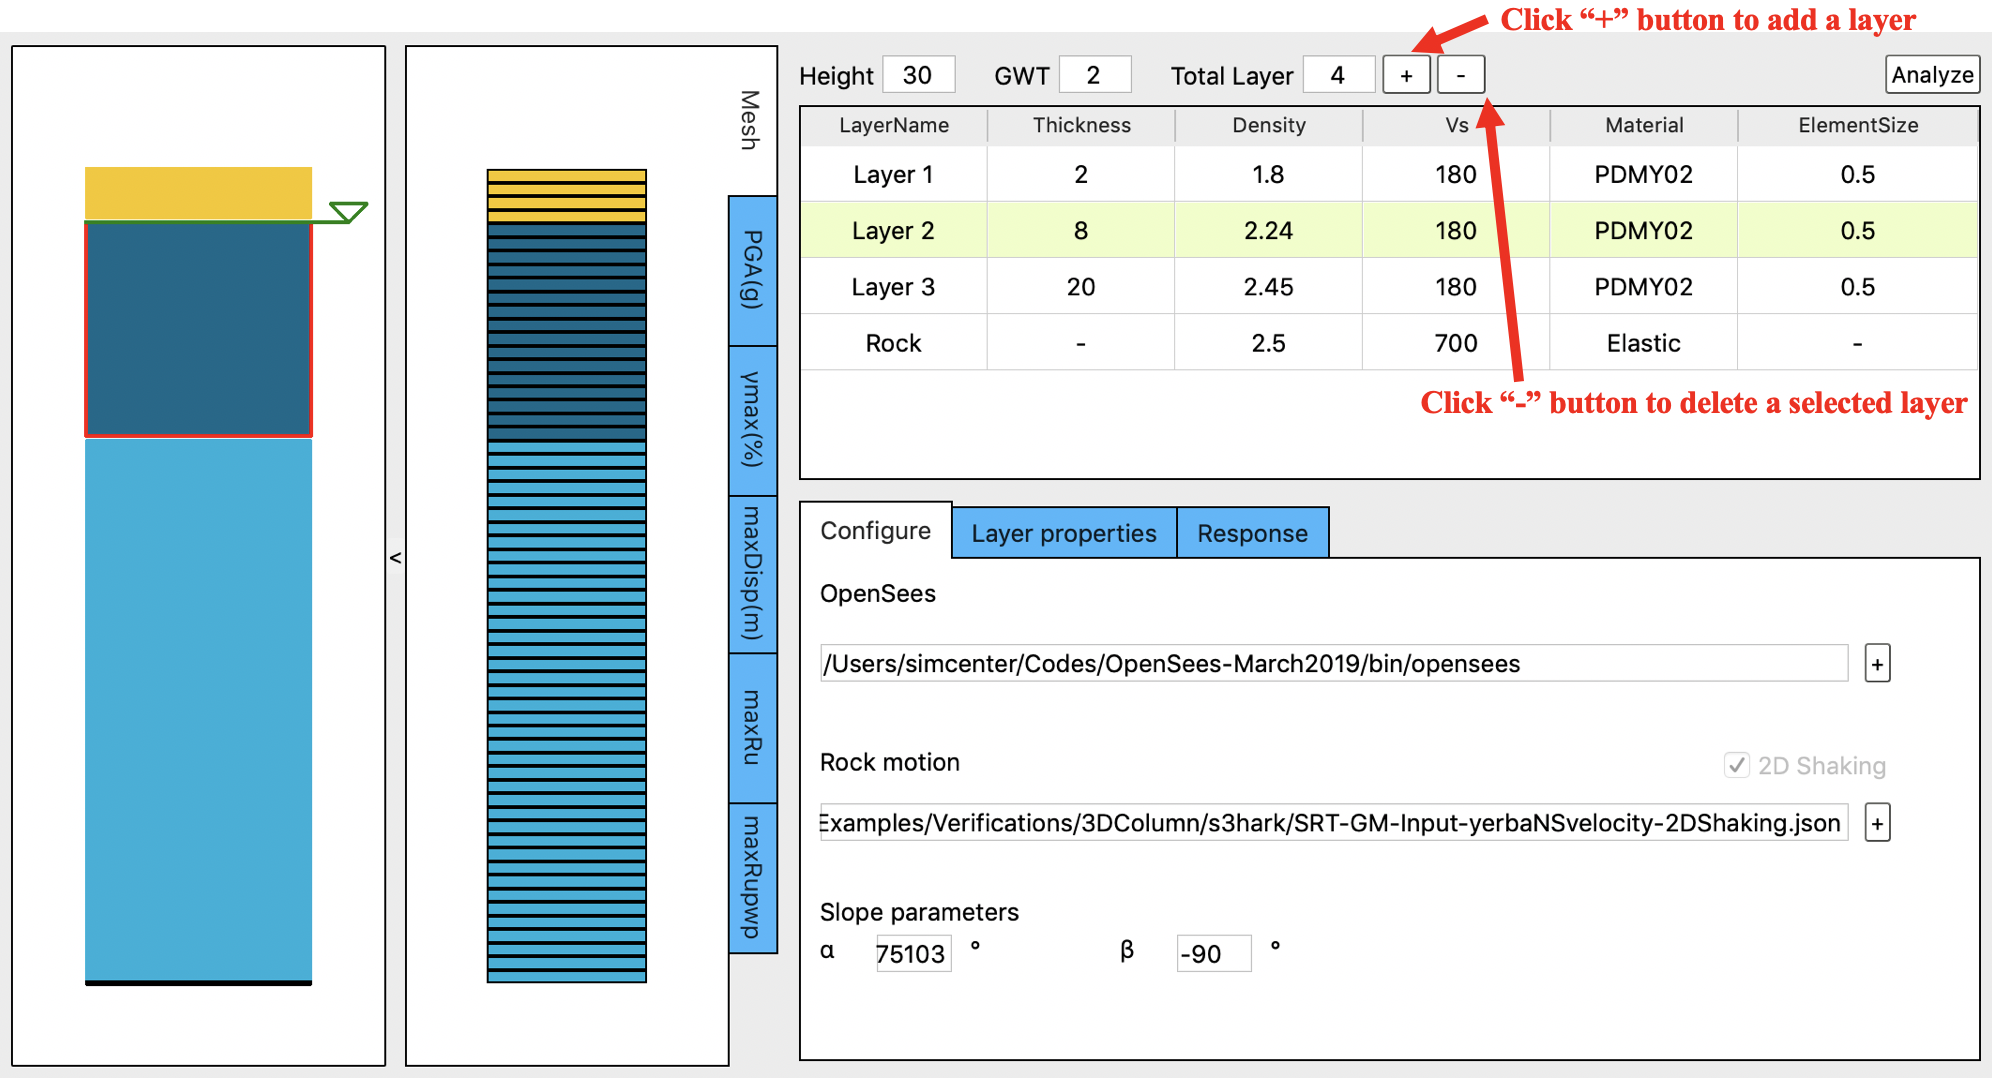
\includegraphics[width=0.9\textwidth]
    {installation/figures/addLayer.png} }
  \caption{Adding soil layers}
  \label{fig:addLayer}
\end{figure}


Click on the configure tab to show configurations options. 
Under the "OpenSees" label, type the path of OpenSees executable. 
You can also select the executable from your local computer by clicking on the "+" button on the right of the input area (\Cref{fig:addOpenSees}).

Under the "Rock motion" label, type the path of a ground motion file. 
You can also select the file from your local computer by clicking on the "+" button on the right of the input area (\Cref{fig:addOpenSees}).

\begin{figure}[!htbp]
  \centering {
    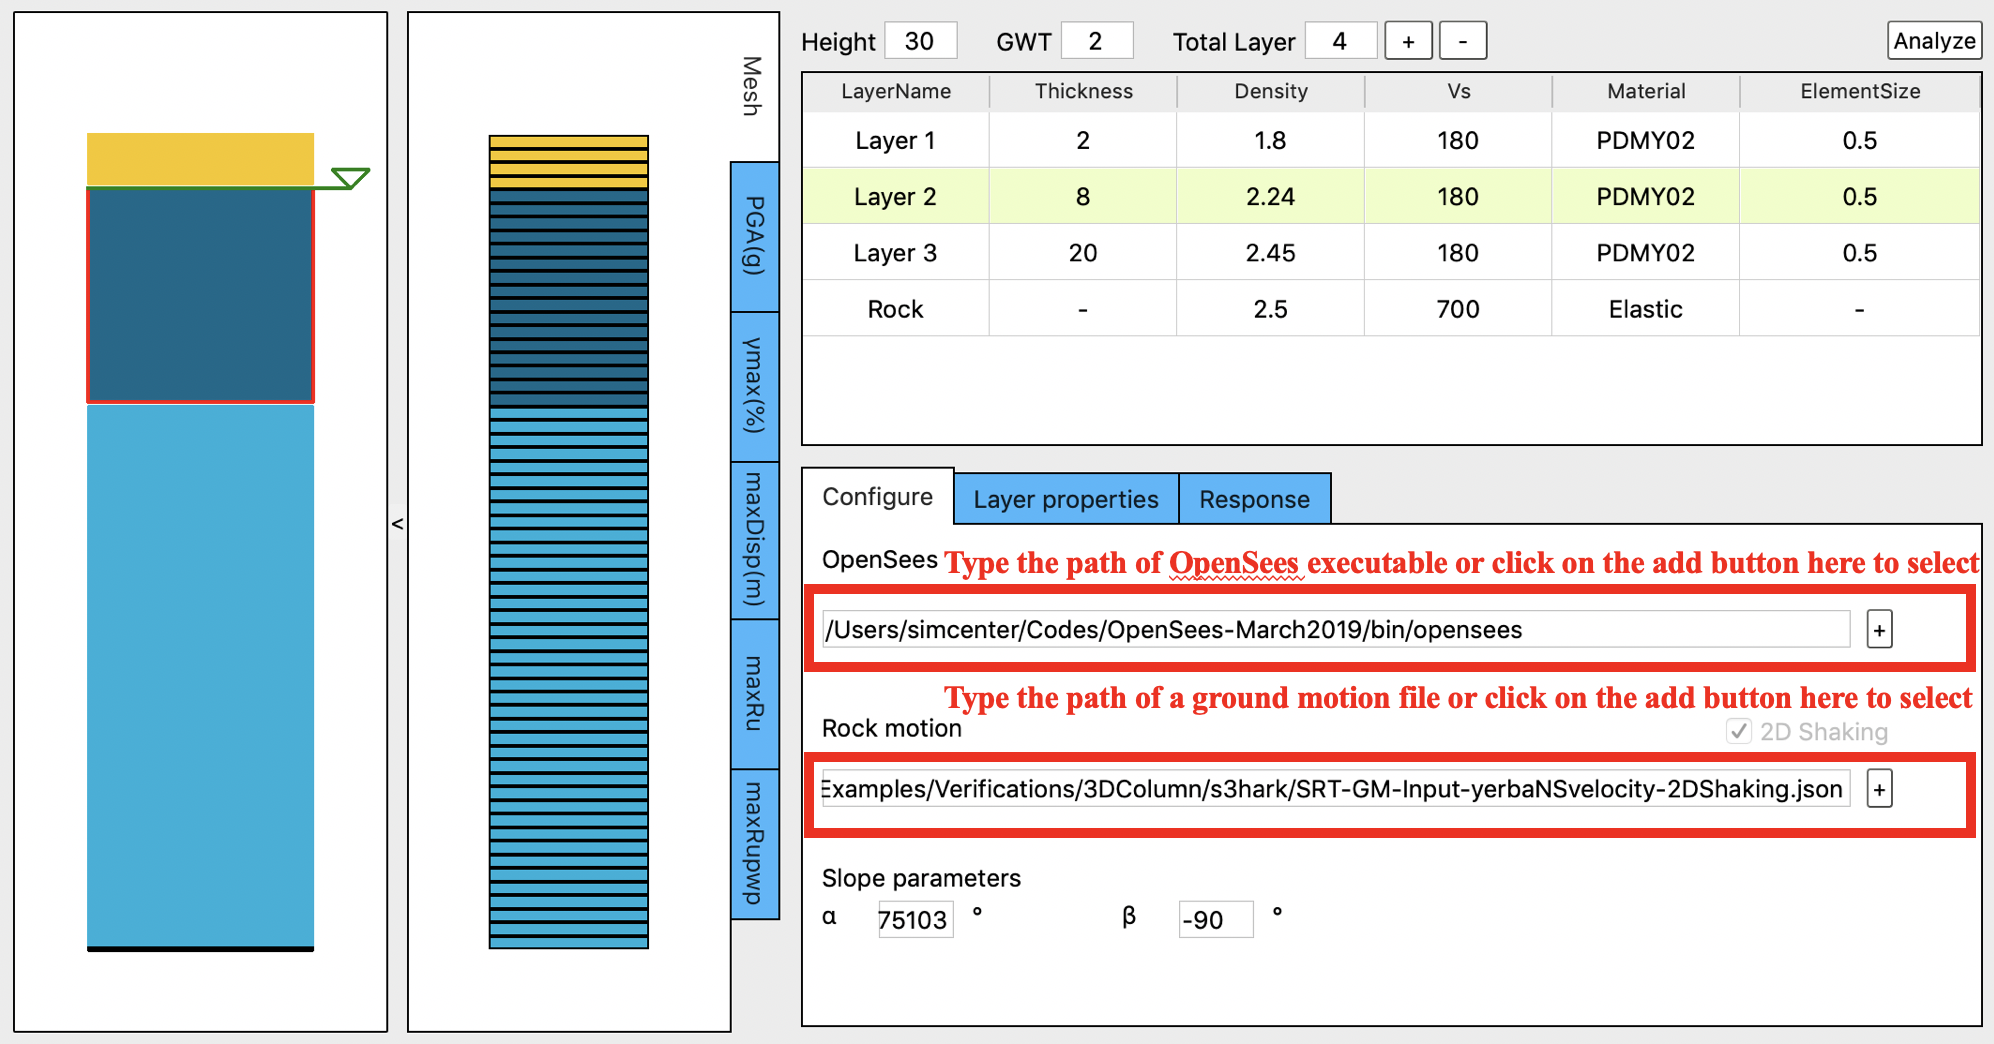
\includegraphics[width=0.9\textwidth]
    {installation/figures/addOpenSees.png} }
  \caption{Adding OpenSees path and rock motion file}
  \label{fig:addOpenSees}
\end{figure}


\begin{figure}[!htbp]
  \centering {
    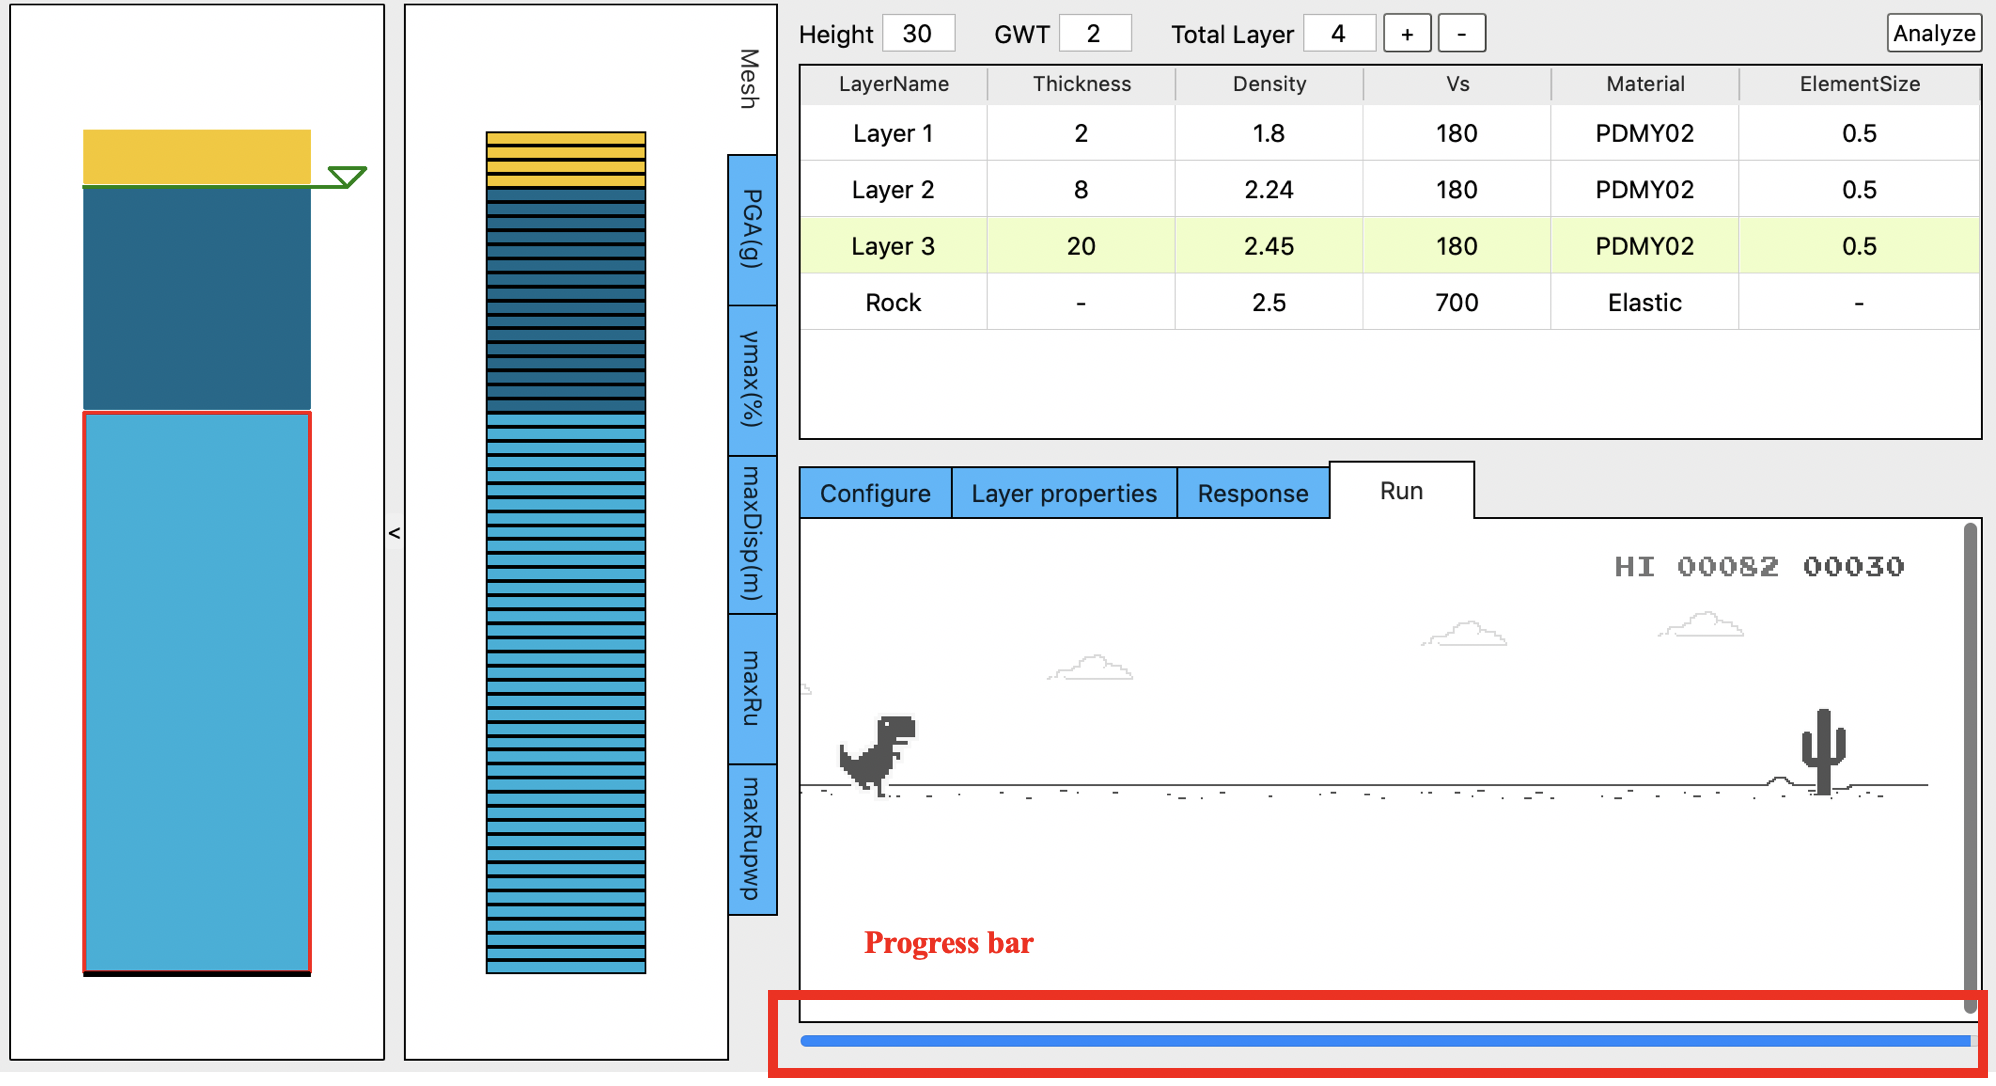
\includegraphics[width=0.9\textwidth]
    {installation/figures/progress.png} }
  \caption{Simulation progress }
  \label{fig:progress}
\end{figure}

Click on the "Analyze" button to run the finite element analysis.
If the soil layers are added successfully, OpenSees path is correct and the rock motion file is correct,
you will see a progress bar (\Cref{fig:prpgress}) displayed at the bottom of the right hand side of the app, which shows the percentage of steps performed. 

\begin{figure}[!htbp]
  \centering {
    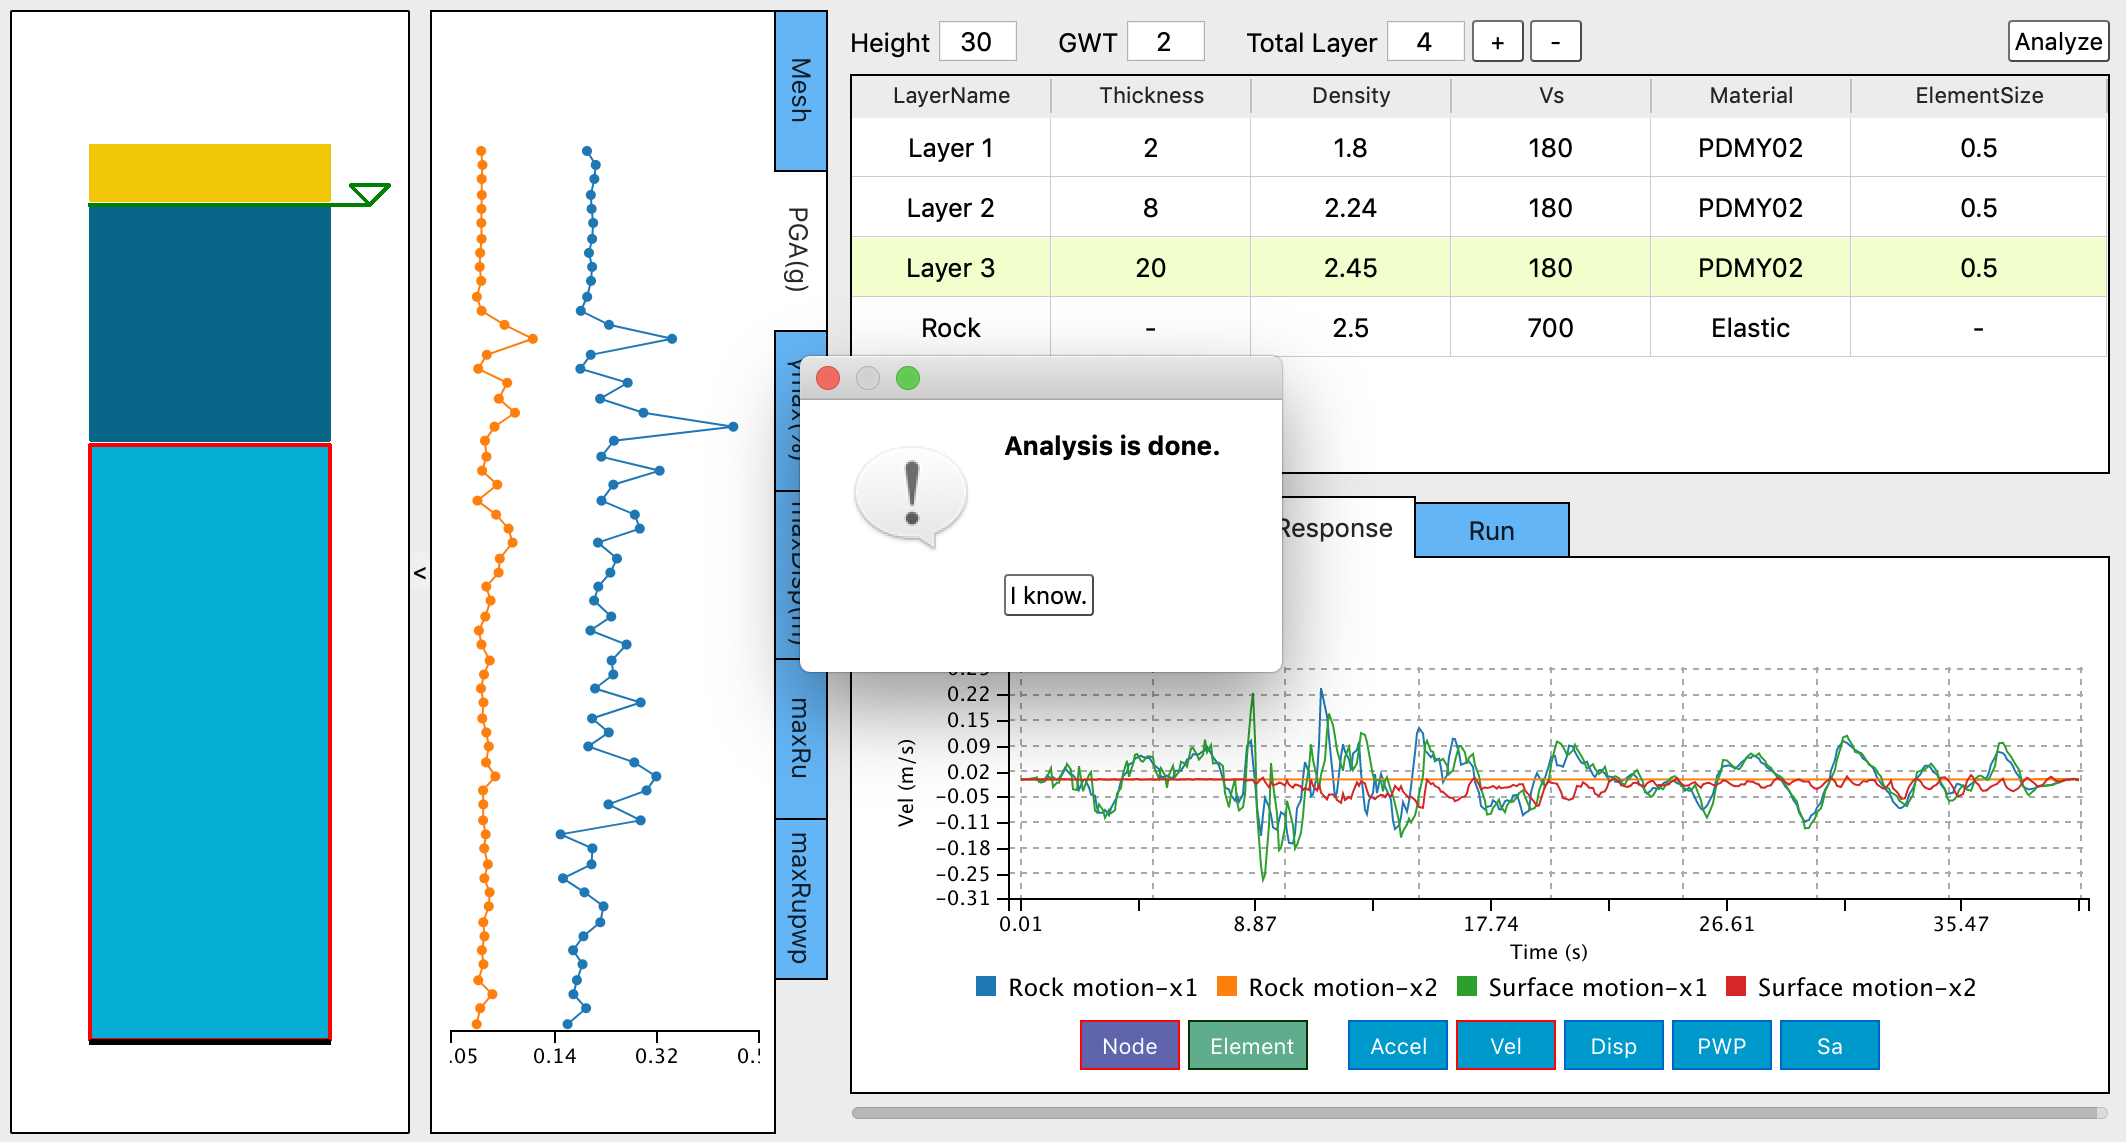
\includegraphics[width=0.9\textwidth]
    {installation/figures/done.png} }
  \caption{Analysis is done }
  \label{fig:done}
\end{figure}

Once the simulation is done, the "Response" tab and the "PGA(g)" profile plot will be displayed.
At the same time, 
a pop up window showing "The analysis is done." will show up.
And when you click "I know.", the progress bar will disappear.

%===============================================================================
